\documentclass[
	12pt,
	]{article}
		\usepackage{xcolor}
			\usepackage[dvipsnames]{xcolor}
			\usepackage[many]{tcolorbox}
		\usepackage{changepage}
		\usepackage{titlesec}
		\usepackage{caption}
		\usepackage{mdframed, longtable}
		\usepackage{mathtools, amssymb, amsfonts, amsthm, bm,amsmath} 
		\usepackage{array, tabularx, booktabs}
		\usepackage{graphicx,wrapfig, float, caption}
		\usepackage{tikz,physics,cancel, siunitx, xfrac}
		\usepackage{graphics, fancyhdr}
		\usepackage{lipsum}
		\usepackage{xparse}
		\usepackage{thmtools}
		\usepackage{mathrsfs}
		\usepackage{undertilde}
		\usepackage{tikz}
		\usepackage{fullpage}
		\usepackage[labelfont=bf]{caption}
	\newcommand{\td}{\text{dim}}
	\newcommand{\tvw}{T : V\xrightarrow{} W }
	\newcommand{\ttt}{\widetilde{T}}
	\newcommand{\ex}{\textbf{Example}}
	\newcommand{\aR}{\alpha \in \mathbb{R}}
	\newcommand{\abR}{\alpha \beta \in \mathbb{R}}
	\newcommand{\un}{u_1 , u_2 , \dots , n}
	\newcommand{\an}{\alpha_1, \alpha_2, \dots, \alpha_2 }
	\newcommand{\sS}{\text{Span}(\mathcal{S})}
	\newcommand{\sSt}{($\mathcal{S}$)}
	\newcommand{\la}{\langle}
	\newcommand{\ra}{\rangle}
	\newcommand{\Rn}{\mathbb{R}^{n}}
	\newcommand{\R}{\mathbb{R}}
	\newcommand{\Rm}{\mathbb{R}^{m}}
	\usepackage{fullpage, fancyhdr}
	\newcommand{\La}{\mathcal{L}}


	\usepackage{mathtools}
	\DeclarePairedDelimiter{\norm}{\lVert}{\rVert}
	\newcommand{\vectorproj}[2][]{\textit{proj}_{\vect{#1}}\vect{#2}}
	\newcommand{\vect}{\mathbf}
	\newcommand{\uuuu}{\sum_{i=1}^{n}\frac{<u,u_i}{<u_i,u_i>} u_i}
	\newcommand{\B}{\mathcal{B}}
	\newcommand{\Ss}{\mathcal{S}}
	
	\newtheorem{theorem}{Theorem}[section]
	\theoremstyle{definition}
	\newtheorem{corollary}{Corollary}[theorem]
	\theoremstyle{definition}
	\newtheorem{lemma}[theorem]{Lemma}
	\theoremstyle{definition}
	\newtheorem{definition}{Definition}[section]
	\theoremstyle{definition}
	\newtheorem{Proposition}{Proposition}[section]
	\theoremstyle{definition}
	\newtheorem*{example}{Example}
	\theoremstyle{example}
	\newtheorem*{note}{Note}
	\theoremstyle{note}
	\newtheorem*{remark}{Remark}
	\theoremstyle{remark}
	\newtheorem*{example2}{External Example}
	\theoremstyle{example}
	
	\title{MATH 325 Ass 4.}
	\titleformat*{\section}{\LARGE\normalfont\fontsize{12}{12}\bfseries}
	\titleformat*{\subsection}{\Large\normalfont\fontsize{10}{15}\bfseries}
	\author{Mihail Anghelici 260928404 }
	\date{\today}
	
	\relpenalty=9999
			\binoppenalty=9999
		
			\renewcommand{\sectionmark}[1]{%
			\markboth{\thesection\quad #1}{}}
			
			\fancypagestyle{plain}{%
			  \fancyhf{}
			  \fancyhead[L]{\rule[0pt]{0pt}{0pt} Assignment 4} 
			  \fancyhead[R]{\small Mihail Anghelici $260928404$} 
			  \fancyfoot[C]{-- \thepage\ --}
			  \renewcommand{\headrulewidth}{0.4pt}}
			\pagestyle{plain}
			\setlength{\headsep}{1cm}
	\captionsetup{margin =1cm}
	\begin{document}
	\maketitle
		\section*{Question 1}
			\subsection*{a) }
				\begin{align*}
					\La [t^{p}] &= \int_{0}^{\infty} e^{-st}t^{p} \ dt 
					\intertext{Let $r=st \implies dt = dr/s$ such that }
					&= \int_{0}^{\infty} e^{-r}\left(\frac{r}{s}\right)^{p} \\
					&= \int_{0}^{\infty} \frac{e^{-r}r^{p}}{s^{p}} \frac{dr}{s}= \frac{1}{s^{p+1}} \int_{0}^{\infty }e^{-r}r^{p} \ dr
					\intertext{Since $\Gamma (p+1) \equiv  \int_{0}^{\infty}e^{-r}r^{p} dr$ , }
					\implies \La[t^{p}]&= \frac{\Gamma (p+1)}{s^{p+1}}, \quad s>0.
				\end{align*}
			\subsection*{b) }
				Let us prove the claim using mathematical induction. Let us assume that $\La [t^{n}] = \dfrac{n!}{s^{n+1}}$.
				\begin{itemize}
					\item Base case \textbf{($n=0$)}: 
					$$ \La [t^{0}] = \La [1] = \frac{1}{s} = \frac{0!}{s^{0+1}} \ \  \quad ,s>0 \quad \checkmark.$$
					\item Inductive step \textbf{($n=n+1$)}:
					\begin{align*}
						\La[t^{n+1}] &= \int_{0}^{\infty } t^{n+1}e^{-st} \ dt 
						\intertext{Applying integration by parts with $u = t^{n+1}$ and $dv = e^{-st}$ yields}
						&= \eval{\frac{e^{-st}}{-s}t^{n+1}}_{0}^{\infty} + \int_{0}^{\infty} \frac{e^{-st}}{s} (n+1) t^{n} \ dt \\
						&= (0 - 0) + \left(\frac{n+1}{s}\right) \int_{0}^{\infty} e^{-st} t^{n} \ dt= \left(\frac{n+1}{s}\right)\La[t^{n}]\\ 
						\La [t^{n+1}] &= \frac{n+1}{s} \frac{n!}{s^{n+1}} = \frac{(n+1)!}{s^{n+2}} \ \ \quad ,s>0 \quad  \checkmark.
					\end{align*}
				\end{itemize}
				We conclude that the initial assumption is true since both cases are satisfied.
			\subsection*{c) }
				\begin{align*}
						\La[t^{-1/2}] &= \int_{0}^{\infty} e^{-st} t^{-1/2} \ dt.
						\intertext{Letting $u = st \implies du/s = dt$ , therefore} 
							&=\int_{0}^{\infty} e^{-u}\left(\frac{u}{s}\right)^{-1/2} \frac{du}{s} = \frac{1}{\sqrt{s}} \int_{0}^{\infty} \frac{e^{-u}}{\sqrt{u}} \ du. \quad ,s>0
							\intertext{Letting $\omega = \sqrt{u} \implies \omega^{2} = u $ and $du = 2\omega d\omega$ such that }
							&= \frac{2}{\sqrt{s}} \int_{0}^{\infty} e^{-\omega^{2}} \ d\omega \quad s>0.
							\intertext{We'll use Fubini's theorem to solve the above integrsal ;}
							\frac{2}{\sqrt{s}} \int_{0}^{\infty} e^{-\omega^{2}} \ d\omega &= \frac{2}{\sqrt{s}}\left(\frac{1}{2}\right) \int_{-\infty}^{\infty} e^{-\omega^{2}} \ d\omega 
							= \frac{1}{\sqrt{s}}\left(\iint\limits_{\R^{2}} e^{-(x+y)^{2}} \ dA\right)^{-1/2}.
							\intertext{Using polar coordinates , }
							&= \frac{1}{\sqrt{s}} \left(\int_{0}^{\infty}\int_{0}^{2\pi} e^{-r^{2}} r \ dr d\theta\right)^{-1/2}.
							\intertext{Applying integration by parts once yields}
							&= \frac{1}{\sqrt{s}}\left(-\pi \eval{e^{-w^{2}}}_{0}^{\infty}\right)^{-1/2}  =\frac{1}{\sqrt{s}}\sqrt{\pi} \quad ,s>0 \\
							\therefore \La[t^{-1/2}] &= \sqrt{\frac{\pi}{s}} \quad ,s>0.
				\end{align*}
			\subsection*{d) }
				\begin{align*}
					\La[\sqrt{t}] &= \int_{0}^{\infty}e^{-st}t^{1/2} \ dt 
					\intertext{Letting $u = st \implies dt = du/s$, }
					&=\int_{0}^{\infty} \frac{e^{-u} u^{1/2}}{s^{3/2}} \ du= \frac{1}{s^{3/2}} \La[u^{1/2}]\quad, s>0.
					\intertext{Since $\La[u^{1/2}] = \int_{0}^{\infty} \frac{e^{-u}}{\sqrt{u}} \ du = \int_{0}^{\infty}e^{-w^{2}} \ dw = \sqrt{\pi}/2$, }
					\La[\sqrt{t}] &=\frac{\sqrt{\pi}}{2s^{3/2}} \qquad ,s>0.
				\end{align*}
		\section*{Question 2}
			\subsection*{a) }
				\begin{align*}
					\La [\sin t] &= \La[t] - \frac{\La[t^{3}]}{3!}+ \frac{\La [t^{5}]}{5!} - \dots \\
					&= \frac{1}{s^{2}} - \left(\frac{3!}{3!}\right) \left(\frac{1}{s^{4}}\right) + \left(\frac{5!}{5!}\right)\left(\frac{1}{s^{6}}\right) -\dots \\
					&= \frac{1}{s^{2}} - \frac{1}{s^{4}} + \frac{1}{s^{6}} - \dots \\
					&= \left(\frac{1}{s^{2}}\right)\sum_{n=0}^{\infty} \left(\frac{-1}{s^{2}}\right)^{n}
					= \frac{1}{s^{2}} \left(\frac{1}{1 + \frac{1}{s^{2}}}\right) = \frac{1}{s^{2} + 1},\quad s>1.
				\end{align*}
			\subsection*{b) }
				\begin{equation*}
					\left(\sin(t)\right)\left(\frac{1}{t}\right) = \sin(t) t^{-1} = \sum_{n=0}^{\infty} \frac{(-1)^{n} t^{2n+1}}{(2n+1)!} (t^{-1}) = \sum_{n=0}^{\infty} \frac{(-1)^{n}t^{2n}}{(2n+1)!} \equiv f 
				\end{equation*}
				\begin{align*}
					\La [f] &= \La[1] - \frac{\La[t^{2}]}{3!} + \frac{\La[t^{4}]}{5!} - \dots \\
					&= \frac{1}{s} - \frac{1}{3s^{3}} + \frac{1}{5s^{5}} - \dots = \sum_{n=0}^{\infty} \frac{(-1)^{n} \left(\frac{1}{s}\right)^{2n+1}}{2n+1} = \arctan(1/s) \ \ \ ,s>0
				\end{align*}
		\section*{Question 3}
			\subsection*{a) }
				Let us first compute the Laplace transform of $f(t)$. 
				\begin{align*}
					\La [f(t)] &=  \int_{0}^{10} e^{-st}(1) \ dt + \int_{10}^{\infty}e^{-st}(0) \ dt.
					\intertext{Since there's no area under \int_{0}^{\infty} 0 \ dt,}
					&= \eval{\frac{e^{-st}}{-s}}_{0}^{10} + 0 = \frac{-e^{-10s}}{s} + \frac{1}{s} = \frac{1-e^{-10s}}{s} \ \ \ ,s>0 .
				\end{align*}
				We may now solve the IVP, 
				\begin{align*}
					\La[y'' + 3y' + 2] &= \La[f] \\
					s^{2} Y(s) + 3sY(s) + 2Y(s) &= \frac{1-e^{-10s}}{s} \\
					\implies Y(s) &= \frac{1-e^{-10s}}{s(s^{2} + 3s + 2)}\\
					&=\frac{1}{s(s^2 +3s +2)} - \frac{e^{-10s}}{s(s^2 +3s +2)} \\
					y(t) &= \La^{-1} \bigg[\frac{1}{s}\bigg] \ast \La^{-1} \bigg[\frac{1}{(s+1)(s+2)}\bigg] - \left(\La^{-1}\bigg[\frac{e^{-10s}}{s}\bigg] \ast \La^{-1}\bigg[\frac{1}{(s+1)(s+2)}\bigg] \right) \\
					&=1 \ast \left(\La^{-1}\bigg[\frac{1}{s+1}\bigg] - \La^{-1} \bigg[\frac{1}{s+2}\bigg]\right) \\
					&\hphantom{=} - \left(u_{10}(t) \ast \left(\La^{-1}\bigg[\frac{1}{s+1}\bigg] - \La^{-1}\bigg[\frac{1}{s+2}\bigg]\right)\right) \\
					&= \int_{0}^{\tau} (e^{-\tau}-e^{-2\tau}) \ d\tau - \left(g(t-10)\int_{0}^{\tau}(e^{-\tau} - e^{-2\tau}) \ d\tau\right) \\
					\intertext{Solving the LHS and RHS integral yields}
					y(t) &=\frac{1}{2}- e^{-t} + \frac{e^{-2t}}{2} - \left(\frac{1}{2}-e^{-(t-10)}+\frac{e^{-2(t-10)}}{2}\right)u_{10}(t)
				\end{align*}
			\subsection*{b) }
				\begin{align*}
					\La [y'' + y' + \frac{5y}{4}] &= \La[t-(t-\pi/2)u_{\pi/2}(t)] \\
					Y(s)\left(s^{2} + s + \frac{5}{4}\right) &= \frac{1}{s^{2}} - \frac{e^{\frac{-\pi s}{2}}}{s^{2}} \\
					Y(s) &= \frac{1-e^{\frac{-\pi s}{2}}}{s^{2} \left(s^{2} + s + \frac{5}{4}\right)} \\ 
					&=\frac{1}{s^{2}\left(\left(s+\frac12\right)^{2} + 1\right)} - \frac{e^{\frac{-\pi s}{2}}}{s^{2} \left(\left(s+\frac12\right)^{2} + 1\right)} \\ 
					y(s) &= \La^{-1} \bigg[\frac{1}{s^{2}}\bigg] \ast \La^{-1} \bigg[\frac{1}{\left(\left(s+\frac12\right)^{2} +1\right)}\bigg] \\
					&- \left(\La^{-1} \bigg[e^{\frac{-\pi s}{2}}\bigg] \ast \La^{-1} \bigg[\frac{1}{ \left(\left(s+\frac12\right)^{2} + 1\right)}\bigg] \ast \La^{-1}\bigg[\frac{1}{s^{2}}\bigg]\right) \\
					&= t \ast e^{\frac{-t}{2}} \sin(t) - \left(u_{\pi/2} g(t-\pi/2)\right) \\
					&= \int_{0}^{t} \tau e^{-\tau/2} \sin(\tau)- \left(u_{\pi/2} g(t-\pi/2)\right)
					\intertext{We find $g(t-\pi /2)$ by solving the LHS integral. Let us apply integration by parts with $u = \tau$ and $dv = e^{-\tau /2}\sin(t)$. We must apply another integration by parts to find $v$ such that }
					\int_{0}^{t} e^{-\tau/2}\sin(t) &= \frac{-2}{5} e^{-\tau /2 }(\sin(\tau) + 2 \cos(\tau))
					\intertext{then we apply the initial integration by parts,}
					y(t) &=(4+2t) \frac{e^{\frac{t}{2}} \sin (t)}{5} + \frac{4t}{5} \cos(t) -\left(u_{\pi/2} g(t-\pi/2)\right)
					\intertext{We now express $g(t-\pi/2)$ given the previous result,}
					&=(4+2t) \frac{e^{\frac{t}{2}} \sin (t)}{5} + \frac{4t}{5} \cos(t) -\left(4+2\left(t-\frac{\pi}{2}\right)\right) \frac{e^{\frac{\left(t-\frac{\pi}{2}\right)}{2}} \sin (\left(t-\frac{\pi}{2}\right))}{5}u_{\pi/2}(t)\\
					&\hphantom{=} \  - \frac{4\left(t-\frac{\pi}{2}\right)}{5} \cos(t-\frac{\pi}{2})u_{\pi/2}(t)
				\end{align*}
		\section*{Question 4}
			\subsection*{a) } 
			 	\begin{align*}
			 		\intertext{Let us multiply by $(s-r_{k})$ on both sides yielding} 
			 		\frac{A_{1}}{s-r_{1}}(s-r_{k}) + \dots + \frac{A_{n}}{s-r_{n}} (s-r_{k}) &= \frac{P(s)}{Q(s)}(s-r_{k}) 
			 		\intertext{Since $Q'(s) = (s-r_{k})Q(s)$, }
			 		&=\frac{P(s)}{Q'(s)} 
			 		\intertext{Taking the limit as $s$ approaches $r_{k}$, }
			 		\lim\limits_{s\to r_{k}}(s-r_{k})\frac{P(s)}{Q(s)} = \frac{P(r_{k})}{Q'(r_{k})} = 0 + 0 + \dots + &\frac{A_{k}}{r_{k} - r_{k}} (r_{k} - r_{k}) + 0 +\dots +0 = A_{k}
			 	\end{align*}
			 \subsection*{b) }
			 	\begin{align*}
			 		\La^{-1} \bigg[F(s)\bigg] &= \La^{-1} \bigg[\frac{P(s)}{Q(s)}\bigg] = A_{1} \La^{-1} \bigg[\frac{1}{s-r_{1}}\bigg] + \dots + A_{n}\La^{-1}\bigg[\frac{1}{s-r_{n}}\bigg] \\
			 		&=A_{1} e^{r_{1}t} + \dots + A_{n} e^{r_{n}t} =\sum_{k=1}^{n} A_{k}e^{r_{k}t} = \sum_{k=0}^{n} \frac{P(r_{k})}{Q'(r_{k})} e^{r_{k}t}.
			 	\end{align*}
		\section*{Question 5}
			\subsection*{a) }
				\begin{align*}
					\La[y'' + ty] &= \La[0] \\
					s\La[y'] - y'(0) - \dv{}{s} \La[y] &= 0\\
					s^{2}Y(s) -s -Y'(s) &= 0 \implies Y'(s) -s^{2}Y(s) =-s
				\end{align*}
			\subsection*{b) }
				\begin{align*}
					\La[(1-t^{2})y'' - 2ty' +\alpha(\alpha+1)y] &= \La [0] \\
					\La[y''] - \La[t^{2} y''] - 2\La[ty'] + \alpha(\alpha+1)\La[y] &= 0  \\
					s^{2}Y(s)-1 - \dv[2]{(s^{2}Y(s) -1)}{s} + 2 \dv{(sY(s))}{s} +\alpha(\alpha+1)Y(s) &= 0
					\intertext{Using the product rule on both terms and recollecting everything yields}
					s^{2} Y(s) -1 - s^2 Y''(s) - Y'(s) 4s - Y(s)2 + 2Y(s) + 2sY'(s) + \alpha(\alpha +1)Y(s) &= 0 \\
					\therefore s^2 Y''(s) +2sY'(s) -(s^{2} + \alpha(\alpha+1))Y(s) &= -1
				\end{align*}
		\section*{Question 6}
			\begin{align*}
				\La[y'] + \La [t] &= \frac12 \La[t^{2}] \La[y] \\
				sY(s) -1 +\frac{1}{s^{2}} &= \frac{Y(s)}{s^{3}} \\
				\therefore Y(s) &= \frac{1- \frac{1}{s^{2}}}{s-\frac{1}{s^{3}}} 
				= \frac{s(s^{2} -1 )}{s^{4} -1} = \frac{s}{s^{2}+1} \quad ,s>0\\
				y(t) &= \La^{-1}\bigg[\frac{s}{s^{2}+1}\bigg] = \cos(t).
			\end{align*}
		\section*{Question 7}
			\subsection*{a) }
				\begin{figure}[H]
					\centering
					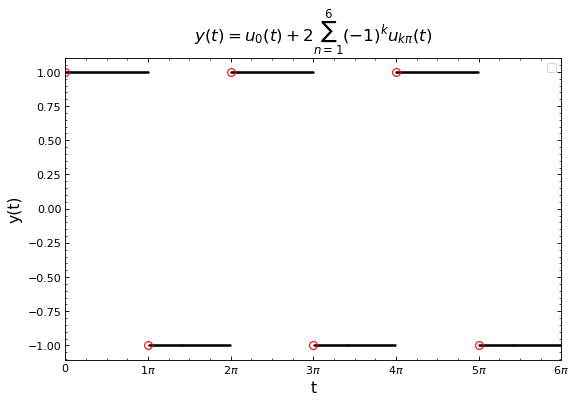
\includegraphics[width=0.8\linewidth]{MATH325_Ass4_Fig1.png}
					\captionsetup{margin=1.5cm, justification=raggedright} \caption{Graph of $f(t)$ for $0 \le t \le 6\pi$.}
				\end{figure}
			\subsection*{b) }
				\begin{align*}
					\La [y''] + \La[y] &= \La[u_{0}(t) + 2\sum_{k=1}^{n} (-1)^{k} u_{k\pi} (t)] \\
					s^{2}Y(s) + Y(s) & = \frac{1}{s} + 2\sum_{k=1}^{n} (-1)^{k} \La[u_{k\pi} (t)] \\
					Y(s) (s^{2} +1 ) &= \frac{1}{s} + 2\sum_{k=1}^{n} (-1)^{k} \frac{e^{-k\pi s}}{s} \\
					Y(s) &= \frac{1}{s(s^{2} +1 )} + 2\sum_{k=1}^{n} (-1)^{k} \frac{e^{-k\pi s}}{s(s^{2}+1)} \quad ,s>0. 
					\intertext{Using partial fraction decomposition on $1/(s(s^{2}+1))$ yields}
					&= \left(\frac{1}{s} - \frac{s}{s^{2}+1}\right) + 2\sum_{k=1}^{n}(-1)^{k} e^{-k\pi s} \left(\frac{1}{s} - \frac{s}{s^{2}+1}\right) \\
					\therefore y(t) &= \La^{-1}\bigg[\frac{1}{s}\bigg] - \bigg[\frac{s}{s^{2}+1}\bigg] + 2\sum_{k=1}^{n} (-1)^{k} u_{k\pi} \La^{-1} [g(t-k\pi)] \\
					&= 1- \cos(t) + 2\sum_{k=1}^{n} (-1)^{k} u_{k \pi}(t) (1-\cos(t-k\pi)).
				\end{align*}
			\subsection*{c) }
				\vspace{-1.75cm}
				\begin{figure}[H]
					\centering 
					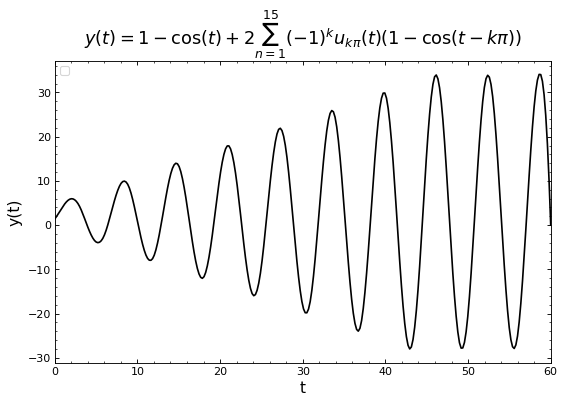
\includegraphics[width=0.8\linewidth]{MATH325_Ass4_Fig2.png}
					\captionsetup{margin=1.5cm , justification=raggedright} \caption{Graph of the solution $y(t)$ for $t \in [0,60]$.}
				\end{figure}
				From Figure 2 we note that the amplitude increases steadily and scales with $y_A = 2y _{0,A}$. This amplitude change is due to the unit step function factor.The amplitude stops increasing at $t = 15\pi$ since the summation is defined up to $n=15$, hence no additional terms are added to the $y(t_{n\ge 15}).$Following this previous remark, we note the solution reaches a steady state at approximately at $t=50$.  Moreover, the function is sinusoidal because of the cosine terms inside the equation. 
			\subsection*{d) }
				As $n$ increases,only the critical point at which the amplitude stops increasing increases linearly with $n$, such that the function's aspect remains identical $\forall n$. As n approaches infinity , $y(t)$ diverges as the sum is alternating series with $b_{n+1} > b_{n} , \ \forall n \ \in \mathbb{N}$, but nevertheless the steady state solution does not change. 
		\section*{Question 8}
			\begin{align*}
				\La[2y'' + y' +4y] &= \La[\delta(t-\pi/6)\sin (t)]\\
				2\La[y'']+\La[y']+4\La[y] &= \sin(-\pi/6) \La[\delta(t-\pi/6)] \\
				Y(s) &= \frac{\sin(-\pi/6)e^{\frac{-\pi s}{6}}}{2\left(s^{2}+\frac{s}{2} + 2\right)} \\
				&=\left(-\frac14\right) \left( \left(\frac{1}{\left(s+\frac14\right)^{2} + \frac{15}{8}}\right) + \left(\frac{e^{\frac{-s\pi}{6}}}{\left(s+\frac14\right)^{2} + \frac{15}{8}}\right)\right)\\
				y(t) &= \left(-\frac{1}{4}\right) \left( \frac{8}{15}\La^{-1}\bigg[\frac{\frac{15}{8}}{\left(s+\frac14\right)^{2} + \frac{15}{8}}\bigg] + \frac{8}{15} \left( \La^{-1}\bigg[e^{\frac{-\pi s}{6}}\bigg] \ast \La^{-1}\bigg[\frac{\frac{15}{8}}{\left(s+\frac14\right)^{2} + \frac{15}{8}}\bigg] \right)\right)\\
				&= \left(-\frac14\right)\left(\frac{8}{15}\right) \left( e^{\dfrac{-t}{4}}\sin(\frac{15t}{8})+ \left( e^{\dfrac{-\left(t-\dfrac{\pi}{6}\right)}{4}}\sin(\frac{15(t-\frac{\pi}{6})}{8})\right)u_{\pi/6}(t)\right)
			\end{align*}
				
			
	\end{document}